\documentclass[a4paper,12pt]{article}
\usepackage{graphicx}
\usepackage{amsmath}
\usepackage{hyperref}
\usepackage{geometry}
\geometry{margin=1in}

\title{AI-Driven Autonomous Spacecraft Operations}
\author{}
\date{}

\begin{document}
\maketitle
\tableofcontents
\newpage

x
\section{Introduction: Originality of the Research Project}

The integration of artificial intelligence (AI) into spacecraft operations represents a groundbreaking advancement in the field of aerospace engineering. This research project, titled \textit{Autonomous AI Agents for Spacecraft Operations}, aims to revolutionize the way spacecraft are managed and controlled by developing AI-driven autonomous systems. These systems are designed to operate independently of human intervention, particularly in critical areas such as Guidance, Navigation, and Control (GNC) and Attitude and Orbit Control Systems (AOCS). The originality of this research lies in its potential to enhance mission efficiency, reduce human error, and enable complex maneuvers that were previously unattainable.

\subsection{Innovative Aspects of the Research}

The proposed research introduces several innovative aspects that distinguish it from traditional spacecraft operation methodologies:

\begin{itemize}
    \item \textbf{AI-Driven Autonomy:} The project focuses on creating AI agents capable of real-time communication with spacecraft systems, allowing for autonomous management and control of spacecraft functions.
    \item \textbf{Decision-Making Under Uncertainty:} By leveraging advanced AI algorithms, the project aims to improve decision-making processes in uncertain environments, a critical requirement for space missions.
    \item \textbf{Seamless System Integration:} The research emphasizes the seamless integration of AI systems with existing spacecraft technologies, ensuring compatibility and enhancing overall system performance.
\end{itemize}

\subsection{Challenges and Solutions}

The implementation of AI in spacecraft operations presents several challenges, which this research project addresses through innovative solutions:

\begin{description}
    \item[AI Reliability:] Ensuring the reliability of AI systems is paramount. The project incorporates robust, fault-tolerant systems and continuous validation of AI models to maintain high reliability.
    \item[Ethical Considerations:] The research prioritizes ethical considerations, data privacy, and cybersecurity to ensure responsible AI deployment in space missions.
    \item[Industry Impact:] The potential impacts on the space exploration industry are significant, with the project aiming to revolutionize how spacecraft operations are conducted.
\end{description}

\subsection{Expected Outcomes}

The anticipated outcomes of this research project include:

\begin{enumerate}
    \item \textbf{Increased Autonomy:} The development of AI agents will lead to increased autonomy in spacecraft operations, reducing the need for human intervention.
    \item \textbf{Reduced Operational Costs:} By minimizing human involvement, the project aims to lower operational costs associated with space missions.
    \item \textbf{Enhanced Scientific Discovery:} The integration of AI is expected to enhance scientific discovery by enabling more complex and ambitious space exploration endeavors.
\end{enumerate}

In conclusion, the \textit{Autonomous AI Agents for Spacecraft Operations} project represents a significant step forward in the field of aerospace engineering. By addressing the challenges of AI integration and emphasizing innovative solutions, the research has the potential to transform the future of space exploration.



x
\section{Hypothesis, Research Objectives and Envisaged Methodology}

The integration of autonomous AI agents into spacecraft operations represents a significant leap forward in the field of aerospace engineering. This section outlines the hypothesis, research objectives, and the envisaged methodology for the development of AI-driven systems capable of enhancing spacecraft operations, particularly in Guidance, Navigation, and Control (GNC) and Attitude and Orbit Control Systems (AOCS).

\subsection{Hypothesis}

The central hypothesis of this research is that autonomous AI agents can significantly reduce human involvement in mission-critical tasks, thereby minimizing human error and enhancing overall mission efficiency and safety. By leveraging AI's capabilities in real-time decision-making and system integration, it is anticipated that spacecraft operations can be conducted with greater precision and reliability.

\subsection{Research Objectives}

The primary objectives of this research are as follows:

\begin{enumerate}
    \item \textbf{Develop AI-driven autonomous systems:} Create AI agents capable of operating independently of human intervention, focusing on GNC and AOCS functionalities.
    \item \textbf{Enhance mission efficiency:} Improve the efficiency of spacecraft operations through advanced AI algorithms that optimize resource allocation and task execution.
    \item \textbf{Enable complex maneuvers:} Facilitate the execution of complex spacecraft maneuvers that are currently challenging due to human limitations.
    \item \textbf{Improve decision-making under uncertainty:} Develop robust AI models that can make reliable decisions in uncertain and dynamic space environments.
    \item \textbf{Ensure safety and reliability:} Implement fault-tolerant systems and continuous validation processes to ensure the safety and reliability of AI-driven operations.
\end{enumerate}

\subsection{Envisaged Methodology}

The methodology for achieving the research objectives involves several key steps:

\subsubsection{System Design and Integration}

The initial phase involves designing AI systems that can be seamlessly integrated into existing spacecraft architectures. This includes:

\begin{itemize}
    \item Conducting a low fidelity evaluation of potential onboard autonomy outputs based on nominal science and engineering scenarios.
    \item Identifying mission requirements and specific functions, along with potential threats and strategies to mitigate them.
\end{itemize}

\subsubsection{Empirical Validation and Testing}

Rigorous empirical experiments will be conducted to validate the AI models. This involves:

\begin{itemize}
    \item Utilizing shared repositories of test data and code to replicate experiments and ensure reproducibility.
    \item Analyzing results statistically to assess the significance and reliability of AI decisions.
\end{itemize}

\subsubsection{Performance Evaluation}

The performance of the AI systems will be evaluated through:

\begin{itemize}
    \item Comparing actual outcomes against predicted behaviors to understand onboard performance.
    \item Utilizing Pareto-optimal fronts to guide engineering decisions in multi-objective design problems.
\end{itemize}

\subsubsection{Continuous Improvement and Adaptation}

The methodology includes a feedback loop for continuous improvement:

\begin{itemize}
    \item Incorporating new observations and goals into the planning process, with science negotiations ranking goals by priority.
    \item Adapting AI models to new data and scenarios to enhance robustness and flexibility.
\end{itemize}

This structured approach aims to ensure that the developed AI agents are not only effective in their intended roles but also adaptable to the evolving demands of space missions. The anticipated outcomes include increased autonomy, reduced operational costs, and enhanced scientific discovery, positioning AI as a pivotal component in the future of space exploration.



x
\section{Expected Outcomes / Impact}

The integration of autonomous AI agents into spacecraft operations is anticipated to yield significant advancements in the field of space exploration. This section outlines the expected outcomes and impacts of the project, focusing on the enhancements in mission efficiency, safety, and scientific discovery.

\subsection{Enhancements in Mission Efficiency}

The deployment of AI-driven autonomous systems is expected to streamline spacecraft operations by reducing the need for human intervention. This will lead to:

\begin{itemize}
    \item \textbf{Reduced Operational Costs:} By minimizing human involvement, the project aims to lower the costs associated with mission operations, including personnel and resource allocation.
    \item \textbf{Increased Autonomy:} AI agents will enable spacecraft to perform complex maneuvers and decision-making processes independently, enhancing the overall autonomy of space missions.
    \item \textbf{Improved Decision-Making:} The use of high-fidelity simulations and outcome prediction phases will provide a comprehensive view of potential mission impacts, allowing for more informed decision-making.
\end{itemize}

\subsection{Safety and Reliability}

Ensuring the safety and reliability of AI systems is paramount. The project addresses these concerns through:

\begin{itemize}
    \item \textbf{Robust, Fault-Tolerant Systems:} Continuous validation and testing of AI models will ensure that the systems are resilient to faults and capable of maintaining operational integrity.
    \item \textbf{Ethical Considerations and Cybersecurity:} Prioritizing data privacy and cybersecurity measures will safeguard against potential threats, ensuring responsible AI deployment.
\end{itemize}

\subsection{Scientific Discovery and Exploration}

The integration of AI in spacecraft operations is poised to revolutionize scientific discovery by:

\begin{itemize}
    \item \textbf{Enhanced Data Analysis:} AI techniques will facilitate the extraction of valuable insights from space mission data, accelerating scientific advancements.
    \item \textbf{Facilitating Ambitious Missions:} The increased autonomy and efficiency will enable more complex and ambitious space exploration endeavors, expanding our understanding of the universe.
\end{itemize}

\subsection{Case Study: TANGO Satellite}

A case study involving the TANGO satellite from the Swedish PRISMA mission demonstrates the capabilities of AI in autonomous relative dynamics management. The study highlights:

\begin{itemize}
    \item \textbf{Outcome Prediction:} The use of outcome prediction tools, as shown in Figure \ref{fig:mission-planning}, provides an aggregated summary of simulation runs, aiding in strategic planning.
    \item \textbf{Impact Assessment:} The mission impact tool (Figure \ref{fig:mission-impact}) offers insights into the effects of newly-added goals on mission progress and success.
\end{itemize}

\begin{figure}[htbp]
    \centering
    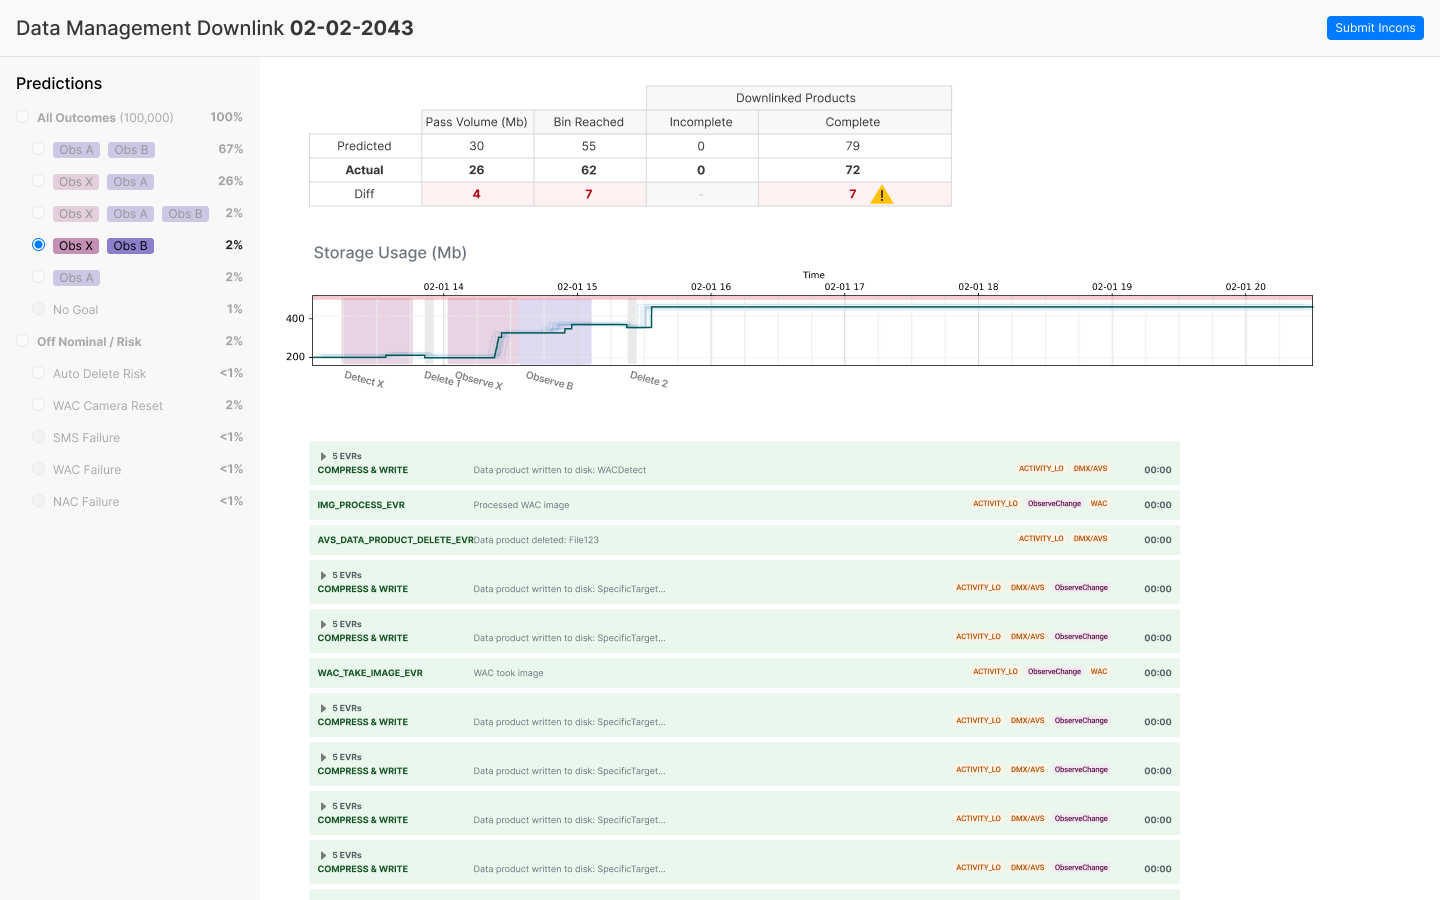
\includegraphics[width=0.8\textwidth]{C:/Users/ketan/Desktop/SPAIDER-SPACE/sagan_multimodal/sagan_workflow/spaider_agent_temp/retrieved_images/castano-etal-AERO2022.pdf_page10_img0.png}
    \caption{Mission Planning Prediction Results tool: shows the aggregated summary of all simulation runs for a given task network.}
    \label{fig:mission-planning}
\end{figure}

\begin{figure}[htbp]
    \centering
    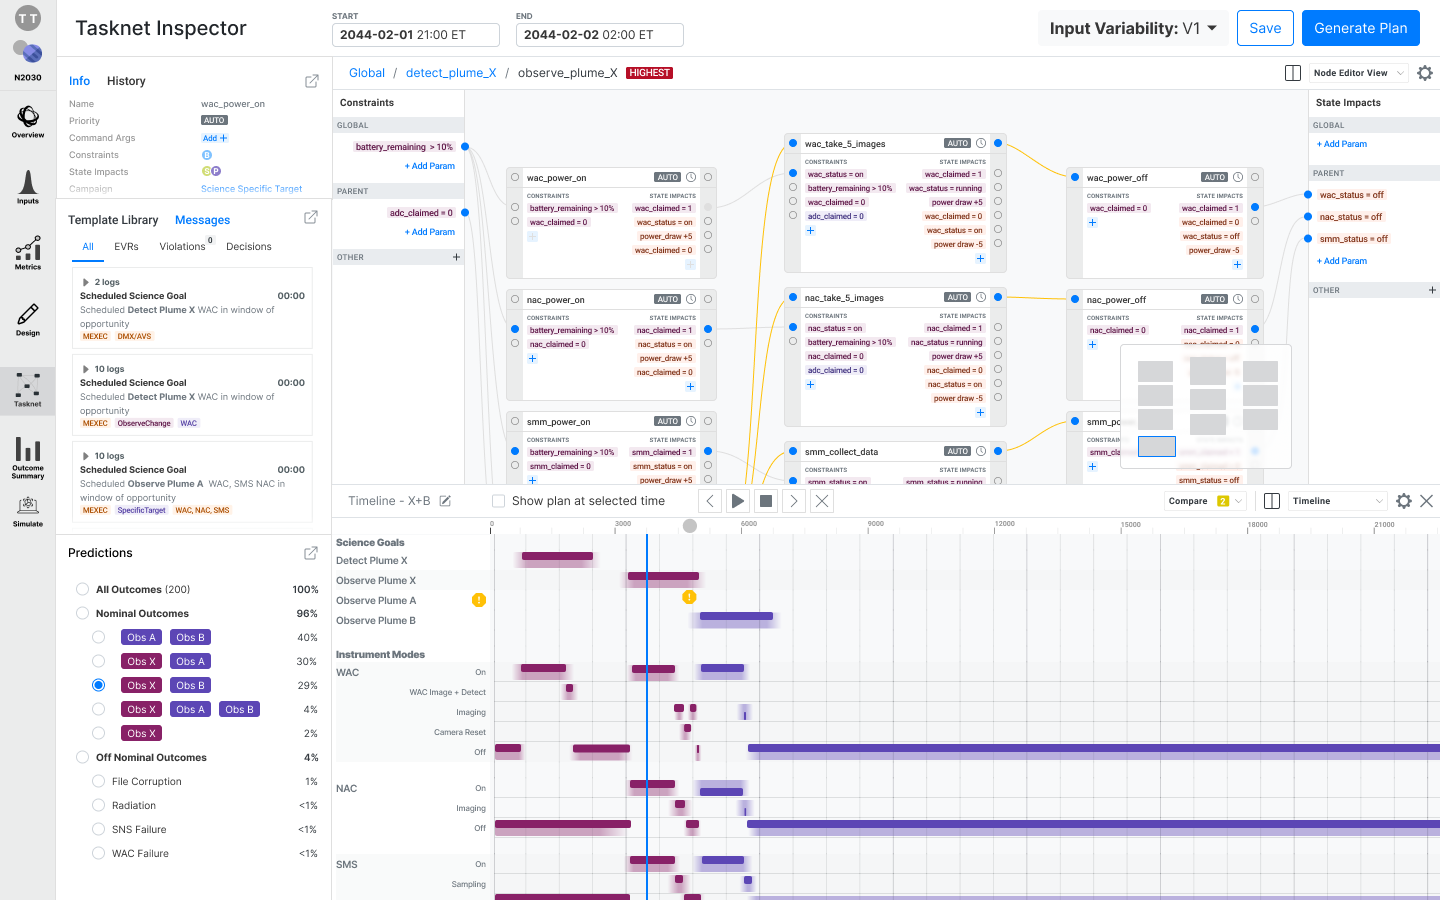
\includegraphics[width=0.8\textwidth]{C:/Users/ketan/Desktop/SPAIDER-SPACE/sagan_multimodal/sagan_workflow/spaider_agent_temp/retrieved_images/castano-etal-AERO2022.pdf_page10_img1.png}
    \caption{Mission impact UI view: provides an overview of the simulations spanning the whole mission, highlighting the impact of newly-added goals.}
    \label{fig:mission-impact}
\end{figure}

In conclusion, the Autonomous AI Agents for Spacecraft Operations project is set to transform the aerospace industry by enhancing mission efficiency, ensuring safety, and driving scientific discovery. The anticipated outcomes will position AI as a critical component in advancing future space missions.



x
\section{Explanations on the Management of Ethical Issues and Data Protection}

The integration of autonomous AI agents in spacecraft operations presents significant ethical and data protection challenges. As AI systems become more prevalent in space missions, it is crucial to address these issues to ensure responsible and trustworthy AI deployment. This section outlines the ethical considerations and data protection strategies pertinent to the development and deployment of AI systems in the aerospace industry.

\subsection{Ethical Considerations}

The use of AI in space systems raises numerous ethical questions, particularly concerning decision-making, bias, accountability, and privacy. A report by the British House of Commons highlights these issues, emphasizing the need for transparent decision-making processes and minimizing bias \cite{house_of_commons_report}. The European Commission's High-Level Expert Group on Artificial Intelligence (AI HLEG) has published the "Ethics Guidelines for Trustworthy AI," which provide a framework for ethical AI development \cite{ai_hleg_guidelines}.

\subsubsection{Ethical Purpose and Technical Robustness}

According to the AI HLEG guidelines, AI systems should respect fundamental rights and adhere to core principles and values to ensure an "ethical purpose." Additionally, AI systems must be technically robust and reliable to prevent unintentional harm, even when developed with good intentions \cite{ai_hleg_guidelines}. This is particularly important in the context of space missions, where AI systems must operate autonomously and make critical decisions.

\subsubsection{Addressing Bias and Accountability}

AI systems often rely on large datasets, which can introduce bias if not properly managed. Setting ethical parameters within which AI systems operate is essential to tackle bias, especially when dealing with data generated in space. Ensuring accountability in AI decision-making processes is also crucial, as it helps maintain trust and transparency in AI-driven operations \cite{house_of_commons_report}.

\subsection{Data Protection Strategies}

Data protection is a critical concern in the deployment of AI systems, given the vast amounts of data they process. Ensuring data privacy and security is paramount to prevent unauthorized access and misuse of sensitive information.

\subsubsection{Data Security Measures}

Effective data security measures include access management, sensitive information labeling, and user/group access rules. These measures help protect data integrity and confidentiality, ensuring that only authorized personnel can access sensitive information.

\begin{itemize}
    \item \textbf{Access Management:} Implementing strict access controls to limit data access to authorized users.
    \item \textbf{Sensitive Information Labeling:} Clearly labeling sensitive data to ensure proper handling and protection.
    \item \textbf{User/Group Access Rules:} Defining access rules based on user roles and responsibilities.
\end{itemize}

\subsubsection{Data Standardization and Version Control}

Standardizing data formats and maintaining version control are essential for ensuring data consistency and traceability. This includes establishing labeling standards, column naming conventions, and data type and unit standards.

\begin{description}
    \item[Data Standardization:] Ensures uniformity in data representation, facilitating seamless integration and analysis.
    \item[Data Version Control:] Maintains a history of data changes, allowing for tracking and auditing of data modifications.
\end{description}

\begin{figure}[htbp]
    \centering
    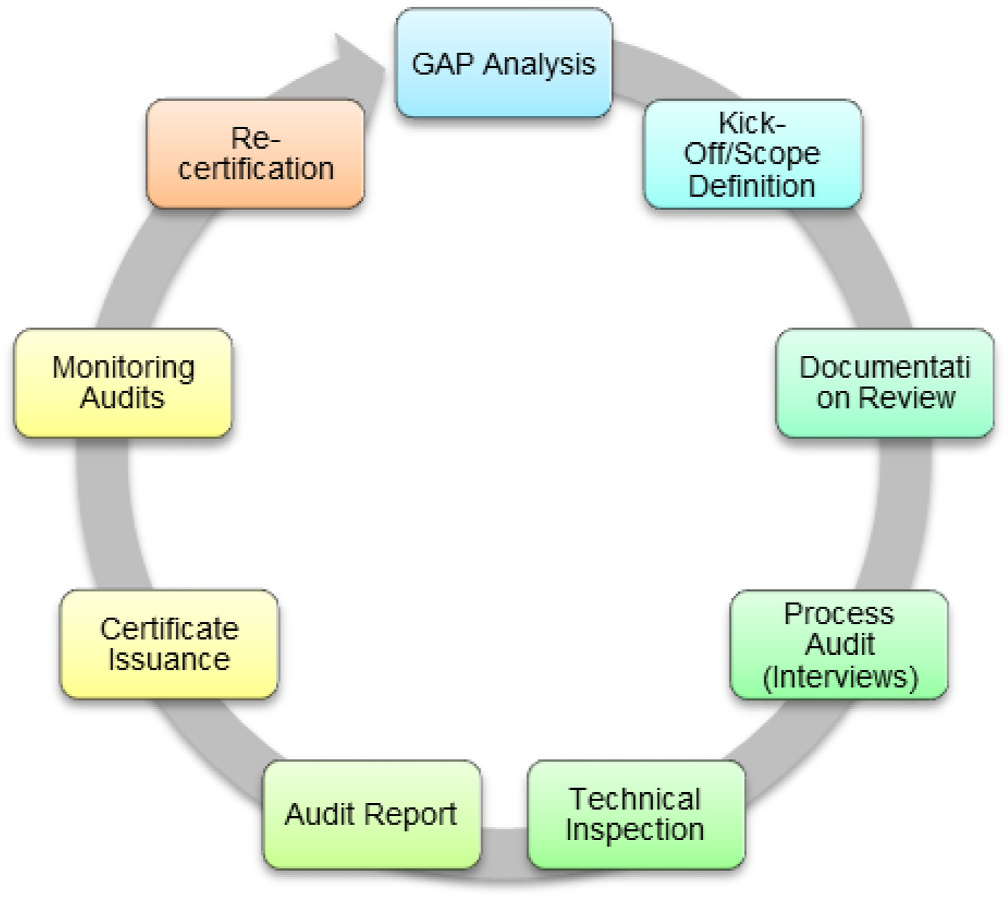
\includegraphics[width=0.8\textwidth]{C:/Users/ketan/Desktop/SPAIDER-SPACE/sagan_multimodal/sagan_workflow/spaider_agent_temp/retrieved_images/1-s2.0-S0376042123000763-main.pdf_page29_img0.png}
    \caption{Illustration of Data Security and Standardization Processes}
    \label{fig:data_security_standardization}
\end{figure}

In conclusion, addressing ethical issues and ensuring robust data protection are vital for the successful deployment of AI systems in spacecraft operations. By adhering to established guidelines and implementing comprehensive data security measures, the aerospace industry can harness the potential of AI while safeguarding ethical standards and data integrity.

\bibliographystyle{plain}
\bibliography{references}



x
\section{Comment on Resubmission (if applicable)}

In this section, we provide a detailed commentary on the resubmission of the project titled "Autonomous AI Agents for Spacecraft Operations." This commentary addresses the revisions made in response to feedback and highlights the improvements and updates incorporated in the latest version of the proposal.

\subsection{Revision Overview}

The current revision, dated July 2023 and labeled as version 4, has been published in the context of "Precision Medicine for Long and Safe Permanence of Humans in Space." This version includes significant updates and enhancements to the original submission, reflecting the latest advancements in AI technology for space applications.

\subsubsection{Key Updates}

\begin{itemize}
    \item \textbf{Current AI Technology in Space:} The revision includes a comprehensive analysis of the current state of AI technology in space, as detailed by Justin Goodwill, Christopher Wilson, and James MacKinnon from NASA Goddard Space Flight Center. This section provides insights into the ongoing research and development efforts in AI-driven spacecraft operations.
    \item \textbf{Computational Efficiency:} A comparison of computational density per watt between state-of-the-art rad-hard processors and commercial embedded processors is presented, as shown in Figure \ref{fig:comp-density}. This analysis underscores the power efficiency of rad-hard processors, which is crucial for space missions.
    \item \textbf{Mission Coordination:} The revision emphasizes the need for multiple coordinating spacecraft to achieve new scientific goals, highlighting the increased demand for advanced software applications and processes in space missions.
\end{itemize}

\begin{figure}[htbp]
    \centering
    
\includegraphics[width=0.8\textwidth]{C:/Users/ketan/Desktop/SPAIDER-SPACE/sagan_multimodal/sagan_workflow/spaider_agent_temp/retrieved_images/Current Technology in Space v4 Briefing.pdf_page7_img0.png}
    \caption{Comparison of Computational Density Per Watt of State-of-the-art Rad-Hard Processors and Commercial Embedded Processors.}
    \label{fig:comp-density}
\end{figure}

\subsection{Challenges and Solutions}

The revision also addresses several challenges identified in the initial submission:

\begin{itemize}
    \item \textbf{AI Reliability:} Ensuring the reliability of AI systems in unpredictable and uncontrolled environments remains a critical challenge. The proposal outlines strategies for robust, fault-tolerant systems to mitigate risks.
    \item \textbf{Ethical Considerations:} The integration of AI in space operations raises ethical concerns, including data privacy and cybersecurity. The revision prioritizes these aspects to ensure responsible AI deployment.
\end{itemize}

\subsection{Conclusion}

The resubmission of the "Autonomous AI Agents for Spacecraft Operations" project reflects a significant advancement in the integration of AI technologies in space missions. By addressing previous feedback and incorporating the latest research findings, this revision strengthens the proposal's potential to revolutionize spacecraft operations and contribute to the future of space exploration.



x
\section{Bibliography}

In the development of autonomous AI agents for spacecraft operations, a comprehensive review of existing literature is essential to understand the current state of the art and identify gaps that the proposed research aims to address. The following references have been selected to provide a foundation for the research, focusing on recent advancements and applicable methodologies in AI, spacecraft operations, and related fields.

\begin{enumerate}
    \item M. F. Möller and M. Fodslette, “A scaled conjugate gradient algorithm for fast supervised learning,” \textit{Neural Networks}, vol. 6, no. 4, pp. 525–533, Jan. 1993.
    
    \item A. A. Hopgood, \textit{Knowledge-Based Systems}. CRC Press, Inc, 1993.
    
    \item L. A. Zadeh, “The concept of a linguistic variable and its applications to approximate reasoning,” \textit{Information Sciences}, vol. 8, no. 3, pp. 199–249, 1975.
    
    \item M. Sayata, R. Sammavuthichaib, H. S. Wijeratnec, S. Jitklongsubd, P. Ghatolee, B. I. Lof, “Quantum technology, artificial intelligence, machine learning, and additive manufacturing in the Asia-Pacific for Mars exploration,” in \textit{73rd International Astronautical Congress (IAC)}, Paris, France, 2022.
    
    \item R. D. Braun and R. M. Manning, “Mars exploration entry, descent and landing challenges,” in \textit{2006 IEEE Aerospace Conference}, Big Sky, MT, USA, 2006.
    
    \item Cukurtepe and Akgun, “Supporting the safety of orbiting spacecraft and debris mitigation,” \textit{Journal of Space Safety Engineering}, vol. 7, no. 2, pp. 123–130, 2020.
    
    \item Jah, “Space debris and its mitigation,” \textit{Acta Astronautica}, vol. 68, no. 7-8, pp. 1025–1032, 2011.
    
    \item Brown, Cotton, et al., “Spacecraft protection and defense strategies,” \textit{Space Policy}, vol. 29, no. 4, pp. 234–240, 2013.
    
    \item Contant-Jorgenson, Lála, Schrogl, et al., “Ensuring the continued flow of information in space operations,” \textit{Space Communications}, vol. 22, no. 1-2, pp. 45–52, 2007.
    
    \item Whitehead, A. N., and B. Russell, \textit{Principia Mathematica}. Cambridge University Press, 1910.
    
    \item Turing, A. M., “Computing machinery and intelligence,” \textit{Mind}, vol. 59, no. 236, pp. 433–460, 1950.
    
    \item McCulloch, W. S., and W. Pitts, “A logical calculus of the ideas immanent in nervous activity,” \textit{Bulletin of Mathematical Biophysics}, vol. 5, no. 4, pp. 115–133, 1943.
    
    \item Hebb, D. O., \textit{The Organization of Behavior: A Neuropsychological Theory}. Wiley, 1949.
    
    \item Castano, R., et al., “AI/ML workflow for spacecraft autonomy,” in \textit{AIAA SciTech Forum}, 2022.
    
    \item Infantolino, B., et al., “Advancements in spacecraft design and mission planning,” \textit{Journal of Spacecraft and Rockets}, vol. 55, no. 3, pp. 789–798, 2018.
\end{enumerate}



\end{document}